\def\BackBleedLeft{204.406}\def\BackGridStart{240.406}
\def\BackContentLeft{246}\def\BackRuleRight{380}
\def\PhotoRight{354}\def\PhotoCenter{300}\def\BioLeft{374}
\def\BarcodeLeft{676.547}
\def\BarcodeGraphic{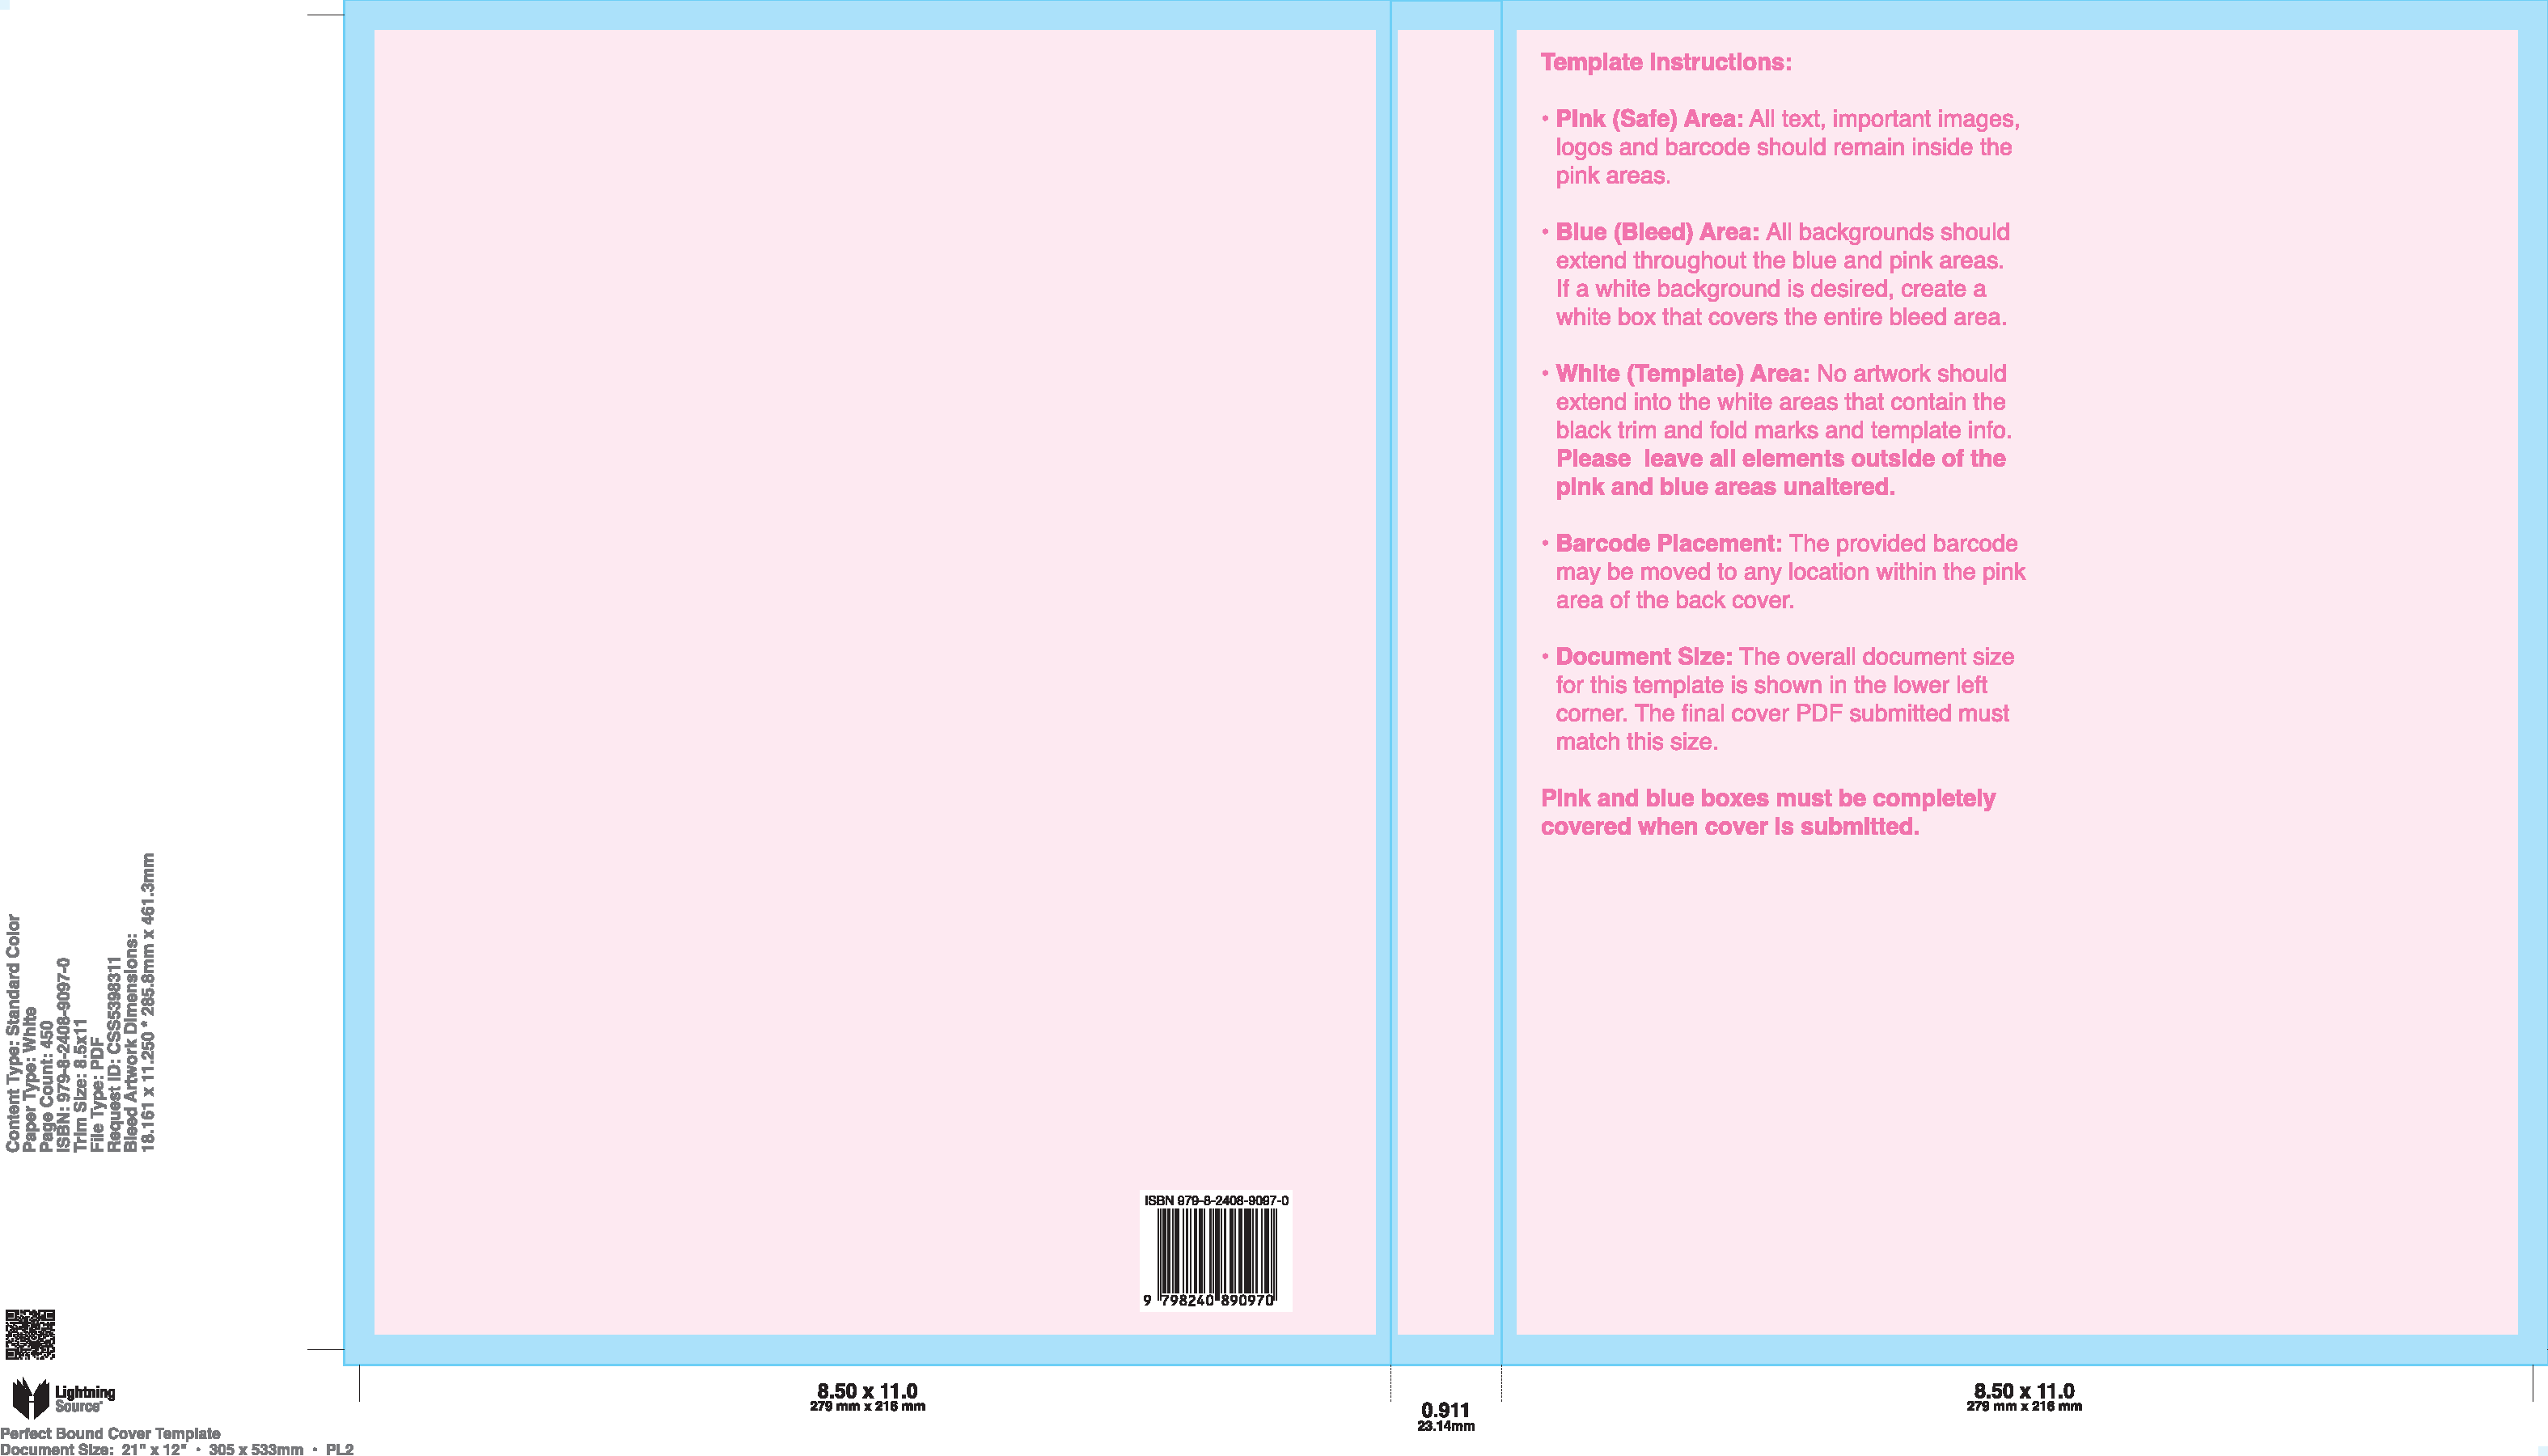
\includegraphics[viewport=676.547 85.695 766.907 157.695,clip,width=90.36pt,height=72pt]{../../templates/9798240890970-Perfect.pdf}}
\def\SpineCenter{858.184}\def\SpineTitleSize{9.2}\def\SpineLeading{10.5}
\def\SpineTitle{SOFTWARE ENGINEERING FOUNDATIONS AND DESIGN}
\def\VolumeLabel{VOLUME I}\def\Accent{cyan}
\def\TitleSize{37}\def\TitleLeading{41}\def\TitleRuleY{547}\def\EditionY{523}
\def\FrontTitle{Software Engineering\par Foundations and Design}
\def\BackHeadline{Build software as an engineered system.}
\def\BackCopy{Software Engineering Foundations and Design provides a practical, systems-oriented introduction to the principles and professional practices that shape modern software development.\\[7pt]
Beginning with software-engineering foundations and the software development lifecycle, the book moves through requirements engineering, UML and systems modeling, software architecture and design patterns, UI/UX design, Agile development, version control, testing, and quality assurance.\\[7pt]
Examples, diagrams, terminal demonstrations, review questions, exercises, and project-based activities connect engineering concepts to professional practice.\\[7pt]
Designed for students, instructors, developers, analysts, and aspiring software engineers, Volume I establishes the foundation for building reliable, maintainable, usable, and high-quality software systems.}
\def\CoverMotif{\begin{scope}[shift={(984,238)},draw=cyan,line width=1.6pt]
\foreach \x/\y in {0/90,80/145,80/35,170/145,170/35,260/90,350/145,350/35,455/90}\fill[navy2,draw=cyan,rounded corners=3pt](\x-18,\y-18)rectangle(\x+18,\y+18);
\draw(18,90)--(62,90)--(80,127);\draw(18,90)--(62,90)--(80,53);\draw(98,145)--(152,145);\draw(98,35)--(152,35);\draw(188,145)--(242,100)--(260,90);\draw(188,35)--(242,80)--(260,90);\draw(278,90)--(332,145);\draw(278,90)--(332,35);\draw(368,145)--(437,90);\draw(368,35)--(437,90);
\foreach \x/\y/\n in {0/90/REQ,80/145/UML,80/35/UI,170/145/ARCH,170/35/CODE,260/90/VCS,350/145/TEST,350/35/QA,455/90/SYSTEM}\node[text=ice,font=\fontsize{7}{8}\selectfont]at(\x,\y){\n};\end{scope}}
\documentclass{article}
\usepackage[paperwidth=21in,paperheight=12in,margin=0in]{geometry}
\usepackage{graphicx,tikz,xcolor,fontspec}
\usetikzlibrary{calc}
\pagestyle{empty}
\setmainfont{TeX Gyre Heros}
\definecolor{navy}{cmyk}{1,0.82,0.32,0.68}
\definecolor{navy2}{cmyk}{0.96,0.76,0.28,0.55}
\definecolor{blue}{cmyk}{0.92,0.67,0,0.10}
\definecolor{cyan}{cmyk}{0.72,0.02,0,0}
\definecolor{ice}{cmyk}{0.10,0.02,0,0}
\definecolor{white}{cmyk}{0,0,0,0}
\definecolor{redaccent}{cmyk}{0.08,0.92,0.62,0.20}
\begin{document}
\noindent\begin{tikzpicture}[remember picture,overlay,x=1pt,y=1pt]
\begin{scope}[shift={(current page.south west)}]
  % Full official bleed rectangles; coordinates come from the supplied template.
  \fill[navy] (\BackBleedLeft,54.0977) rectangle (825.406,864);
  \fill[navy2] (825.386,54.0977) rectangle (890.980,864);
  \fill[navy] (891,54.0977) rectangle (1512,864);
  \begin{scope}[opacity=.10]
    \foreach \x in {\BackBleedLeft,\BackGridStart,...,1512} \draw[cyan,line width=.35pt] (\x,54.0977)--(\x,864);
    \foreach \y in {54.0977,90.0977,...,864} \draw[cyan,line width=.35pt] (\BackBleedLeft,\y)--(1512,\y);
  \end{scope}

  % Back cover: all foreground objects are conservatively inset from the safe box.
  \node[anchor=north west,text=cyan,font=\bfseries\fontsize{10}{12}\selectfont] at (\BackContentLeft,814)
    {THE COMPLETE SOFTWARE ENGINEERING LIFECYCLE · \VolumeLabel};
  \draw[\Accent,line width=3pt] (\BackContentLeft,790)--(\BackRuleRight,790);
  \node[anchor=north west,text=white,text width=516pt,align=left,font=\bfseries\fontsize{19}{23}\selectfont] at (\BackContentLeft,766)
    {\BackHeadline};
  \node[anchor=north west,text=ice,text width=516pt,align=left,font=\fontsize{10.3}{14.1}\selectfont] at (\BackContentLeft,704)
    {\BackCopy};

  \node[anchor=north west,text=cyan,font=\bfseries\fontsize{9.3}{11}\selectfont] at (\BackContentLeft,372) {ABOUT THE AUTHOR};
  \begin{scope}
    \clip[rounded corners=4pt] (\BackContentLeft,246) rectangle (\PhotoRight,354);
    \node[anchor=center,inner sep=0] at (\PhotoCenter,300)
      {
\includegraphics[width=155pt]{../../cover/assets/moody-amakobe-cmyk.jpg}};
  \end{scope}
  \draw[cyan,line width=.8pt,rounded corners=4pt] (\BackContentLeft,246) rectangle (\PhotoRight,354);
  \node[anchor=north west,text=white,font=\bfseries\fontsize{12}{14}\selectfont] at (\BioLeft,352) {Moody Amakobe};
  \node[anchor=north west,text=ice,text width=350pt,align=left,font=\fontsize{8.15}{10.6}\selectfont] at (\BioLeft,329)
    {Moody Amakobe is an academic, applied researcher, and technology professional with extensive experience in software engineering, systems architecture, artificial intelligence, and graduate computing education. He holds a Doctor of Computer Science from Colorado Technical University and has held senior engineering and architecture roles with T-Mobile, Accenture, Wipro, and Deloitte. His teaching and research focus on connecting rigorous computing concepts with real-world engineering practice.};
  \node[anchor=south west,text=cyan,font=\bfseries\fontsize{8.4}{10}\selectfont] at (\BackContentLeft,206)
    {OPEN EDUCATIONAL RESOURCE · CC BY 4.0};
  \node[anchor=south west,text=ice,font=\fontsize{8.4}{10}\selectfont] at (\BackContentLeft,184)
    {GLOBAL DATA SCIENCE INSTITUTE};

  % Preserve the supplied ISBN-specific barcode as vector content at its official location.
  \node[anchor=south west,inner sep=0] at (\BarcodeLeft,85.695) {\BarcodeGraphic};

  % Spine: centered in the official pink safe spine region.
  \node[rotate=90,text=white,font=\bfseries\fontsize{\SpineTitleSize}{\SpineLeading}\selectfont] at (\SpineCenter,482)
    {\SpineTitle};
  \node[rotate=90,text=cyan,font=\fontsize{8.1}{9.5}\selectfont] at (\SpineCenter,171) {MOODY AMAKOBE};

  % Front cover typography.
  \fill[\Accent] (930,789) rectangle (937,830);
  \node[anchor=north west,text=cyan,font=\bfseries\fontsize{9.7}{11.5}\selectfont] at (956,824)
    {THE COMPLETE SOFTWARE ENGINEERING LIFECYCLE · \VolumeLabel};
  \node[anchor=north west,text=white,text width=500pt,align=left,font=\bfseries\fontsize{\TitleSize}{\TitleLeading}\selectfont] at (956,756)
    {\FrontTitle};
  \draw[\Accent,line width=4pt] (956,\TitleRuleY)--(1128,\TitleRuleY);
  \node[anchor=north west,text=ice,font=\fontsize{11}{13}\selectfont] at (956,\EditionY) {2026 EDITION};

  % Distinct lifecycle abstraction supplied by each volume wrapper.
  \CoverMotif

  \node[anchor=south west,text=white,font=\bfseries\fontsize{19}{22}\selectfont] at (956,135) {Moody Amakobe};
  \node[anchor=south west,text=cyan,font=\fontsize{8.8}{10.5}\selectfont] at (956,105)
    {GLOBAL DATA SCIENCE INSTITUTE};
\end{scope}
\end{tikzpicture}\null
\end{document}

